\subsubsection{openEHR approach}

OpenEHR's focus for modeling is multi-level. The models are developed and sustained by domain experts in their own level \cite{openEHRArchitecture}.

First level is based on the reference model. The reference model corresponds to the stable information model, for example, data types or data structures. All EHR data in any openEHR system obey the model of reference. Only this first level is implemented in software \cite{openEHRArchitecture}.

The next level consists of the archetypes. Archetypes correspond to domain content, for example, measurements of blood pressure or diabetes test results. These archetypes are modeled by clinical professionals or IT experts of the field of healthcare, without any technologic knowledge of the final systems. Archetypes are stored in their own repositories.

The templates constitute the next level. These templates specify sets or archetypes used for a particular purpose, and often correspond to screen forms \cite{openEHRArchitecture}.

The last level is where the artifacts generated from the templates are found \cite{openEHR}. The artifacts, shown in figure 1, are not modeled manually. This means that a model for microbiology only needs to be done once in order to enable the reports, user interface forms, documents and other message formats that will be generated.

\begin{figure}[h]
  \centering
  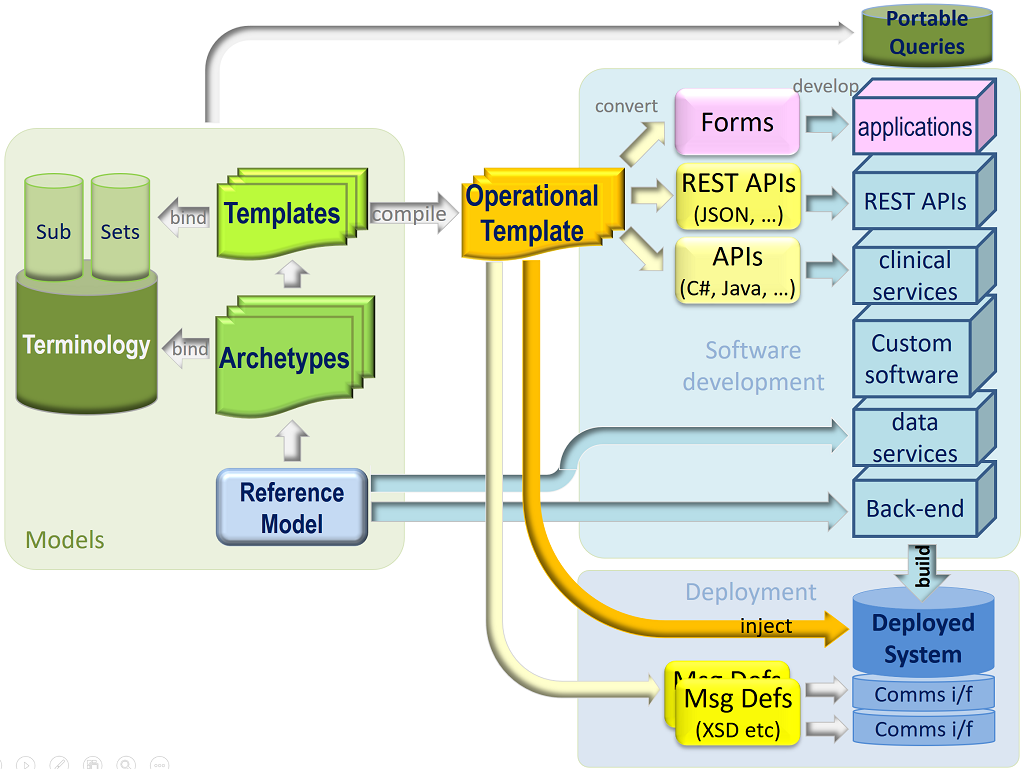
\includegraphics[scale=0.6]{./images/openehr_dev_ecosystem}
  \caption{openEHR approach (Source: extracted from \cite{openEHR}).}
  \label{fig:openeEHR_ecosystem}
\end{figure}
